\documentclass[12pt]{article}
\usepackage{fancyhdr}
%\usepackage{jtygm}
\usepackage{amsmath}
\usepackage{amssymb}
\usepackage{graphicx}
\usepackage{braket}
\usepackage{color}
\usepackage{bm}% bold math
\usepackage{dcolumn}% Align table columns on decimal point

\topmargin=-10mm
\textheight=25cm
\textwidth=17cm
\oddsidemargin=-0.04 cm
\evensidemargin=-1.04cm

\begin{document}
%
% Cover
%
\title{Manual for FermiSurfer\\
version 1.3}
\author{Mitsuaki KAWAMURA}
%\date{}
\maketitle

\tableofcontents

\section{Introduction}

This document is a manual for the Fermi surface drawing program ``Fermi Surfer".
Fermi Surfer have been  developed since 2012 by Mitsuaki Kawamura
(ISSP, The University of Tokyo); 
it is opened on web at November, 2014.
It draws Fermi surfaces, and 
plot $k$-depend matrix elements such as the superconducting gap and
orbital character with colors.

\section{Install}

Requirement
\begin{itemize}
\item C compiler(gcc, intel, PGI, Fujitsu, etc.)
\item GLUT(\texttt{libfreeglut.a}, \texttt{libGL.a}, \texttt{libGLU.a},
 and \texttt{freeglut.h} are required in Linux. 
 \texttt{freeglut.dll} is required in Windows)
\end{itemize}

\subsection{Installation in Linux}

\begin{enumerate}

\item Install the required package

  \begin{itemize}
  \item For Debian/Ubuntu
    \begin{verbatim}
    $ sudo aptitude install freeglut3-dev
    \end{verbatim}
  \item For Red Hat Enterprise Linux/CentOS
    \begin{verbatim}
    $ sudo yum install freeglut-devel.x86_64
    \end{verbatim}
  \end{itemize}

\item Download \verb|fermisurfer.c|

\item Compile

E.g.) gcc 

\begin{verbatim}
  $ gcc fermisurfer.c -fopenmp -O3 -lglut -lGLU -lGL -lm -o fermisurfer
\end{verbatim}

\end{enumerate}

Then a binary file \texttt{fermisurfer} is generated.

\subsection{Installation in Windows}
 
\begin{enumerate}
\item Download the binary \verb|fermisurfer.exe|

\item Download the \verb|zip| file which contains \verb|freeglut.dll|
from ``freeglut Windows Development Library'' site
\begin{verbatim}
http://www.transmissionzero.co.uk/software/freeglut-devel/
\end{verbatim}
(in ``freeglut MSVC package'' item).
Then, \verb|unzip| it.

\item copy \verb|.\bin\freeglut.dll| to the folder which contains
 \verb|fermisurfer.exe|.
 (You should not use \verb|.\bin\x64\freeglut.dll|)

\end{enumerate}

\section{Input file}

\subsection{input-file format}

You have to prepare following data:
\begin{itemize}
\item The number of $k$ grid (three direction)
\item Reciprocal lattice vectors
\item The number of bands
\item The orbital energy at each band and $k$ (We call it ``energy'') .
\item Variables that you want to plot with color (We call it ``matrix elements'').
\end{itemize}

This program supports two kind of uniform $k$ grid,
a grid (${\rm \Gamma}$ centered) and grid with a half-grid shift.
The latter is used when the matrix element becomes singular 
at ${\rm \Gamma}$.

The input file is as follows (\verb|mgb2_vfz.fs|):

\begin{verbatim}
          40          40          36         (1)
           0                                 (2)
           3                                 (3)
   1.0000000      0.57735026      -0.0000000 (4)
   0.0000000       1.1547005       0.0000000 (5)
   0.0000000      -0.0000000      0.87206507 (6)
  2.91340202E-02                             (7)
  2.93242838E-02
  2.98905596E-02
  3.08193434E-02
     :
     :
  0.14393796
  0.12800488
  0.0000000                                  (8)
  0.36269817
  0.71675694
  1.0535113
  1.3644149
     :
     :
  -26.409407
  -19.318560
  -10.315671
\end{verbatim}

\begin{enumerate}
  \renewcommand{\labelenumi}{(\arabic{enumi})}
  \item The $k$ point grid
  \item 0 for ${\rm \Gamma}$centered grid. 1 for shifted grid.
  \item The number of bands
  \item Reciprocal lattice vector 1 (arbitrary unit)
  \item Reciprocal lattice vector 2
  \item Reciprocal lattice vector 3
  \item Energy
  \item Matrix elements
\end{enumerate}

\subsection{How to produce the input file in C and fortran programs}

fortran

\begin{verbatim}
  real(4) :: bvec1(3), bvec2(3), bvec3(3) ! Resiplocal lattice vector
  integer :: nk1, nk2, nk3 ! k-grid of each direction
  integer :: ishift ! 1 for shifted grid, 0 for unshifted grid.
  integer :: nbnd ! The number of bands
  real(4) :: eig(nk3,nk2,nk1,nbnd) ! energy
  real(4) :: x(nk3,nk2,nk1,nbnd) ! matrix element

  integer :: ik1, ik2, ik3, ibnd, fo

  open(fo, file = "sample.fs")
  write(fo,*) nk1, nk2, nk3
  write(fo,*) ishift
  write(fo,*) nbnd
  write(fo,*) real(bvec1(1:3))
  write(fo,*) real(bvec2(1:3))
  write(fo,*) real(bvec3(1:3))
  do ibnd = 1, nbnd
     do ik1 = 1, nk1
        do ik2 = 1, nk2
           do ik3 = 1, nk3
              write(fo,*) real(eig(ik3,ik2,ik1,ibnd)) 
           end do
        end do
     end do
  end do
  do ibnd = 1, nbnd
     do ik1 = 1, nk1
        do ik2 = 1, nk2
           do ik3 = 1, nk3
              write(fo,*) real(x(ik3,ik2,ik1,ibnd)) 
           end do
        end do
     end do
  end do
  close(fo)
\end{verbatim}

C

\begin{verbatim}
  float bvec1[3], bvec2[3], bvec3[3]; /*Resiplocal lattice vector*/
  int nk1, nk2, nk3; /*k-grid of each direction*/
  int ishift; /*1 for shifted grid, 0 for unshifted grid.*/
  int nbnd; /*The number of bands*/
  float eig[nbnd][nk1][nk2][nk3]; /*Energy*/
  float x[nbnd][nk1][nk2][nk3]; /*Matrix element*/

  FILE* fo;
  int ibnd, ik1, ik2, ik3;

  fo = fopen("sample.fs", "w");
  ierr = fprintf(fo, "%d %d %d", nk1, nk2, nk3);
  ierr = fprintf(fo, "%d, iswitch);
  ierr = fprintf(fo, "%d, nbnd);
  ierr = fprintf(fp, "%e %e %e", bvec1[0], bvec1[1], bvec1[2]); 
  ierr = fprintf(fp, "%e %e %e", bvec2[0], bvec2[1], bvec2[2]);
  ierr = fprintf(fp, "%e %e %e", bvec3[0], bvec3[1], bvec3[2]);
  for (ibnd = 0; ibnd < nbnd; ++ibnd) {  
    for (ik1 = 0; ik1 < nk1; ++ik1) { 
      for (ik2 = 0; ik2 < nk2; ++ik2) { 
        for (ik3 = 0; ik3 < nk3; ++ik3) { 
          ierr = fprintf(fo, "%e", eig[ibnd][ik1][ik2][ik3]); 
        } 
      } 
    } 
  } 
  for (ibnd = 0; ibnd < nbnd; ++ibnd) {  
    for (ik1 = 0; ik1 < nk1; ++ik1) { 
      for (ik2 = 0; ik2 < nk2; ++ik2) { 
        for (ik3 = 0; ik3 < nk3; ++ik3) { 
          ierr = fprintf(fo, "%e", x[ibnd][ik1][ik2][ik3]); 
        } 
      } 
    } 
  } 
  fclose(fo); 
\end{verbatim}

\section{Control FermiSurfer}

\subsection{For Linux}
You can launch generated executable as follows:
\begin{verbatim}
$ ./fermisurfer mgb2_vfz.fs
\end{verbatim}
You need a space between the command and input-file name.
(The sample input file \verb|mgb2_vfz.fs| contains
$z$ element of the Fermi velocity in MgB$_2$.)

\subsection{For Windows}
Click mouse right button on the input file.
Choose ``Open With ...'' menu,
then choose \verb|fermisurfer.exe|.

\vspace{0.5cm}
After that, \verb|fermisurfer| runs as the same whether you use Linux or Windows.
The information from the input file is printed.

\begin{verbatim}
#####  Brillouin zone informations  ##### 

k point grid : 40 40 36 
k point grid is not shifted 
# of bands : 3 
bvec 1 : 1.000000 0.577350 -0.000000 
bvec 2 : 0.000000 1.154701 0.000000 
bvec 3 : 0.000000 -0.000000 0.872065 

# of lines for BZ : 84  (1)

#####  Max. and Min. of each bands  ##### 
     
Band   Eig_Min.      Eig_Max      Mat_Min      Mat_Max 
1     -0.428153     0.056262     -24.048639     24.048639 (2)
2     -0.289572     0.121181     -23.320309     23.320309 (2)
3     -0.133566     0.497620     -43.651634     43.651634 (2)

#####  First Brillouin zone mode  #####

band   # of patchs
1       8824  (3)
2       29469 (3)
3       28315 (3)

band   # of nodeline 
1       632   (4)
2       1524  (4)
3       2268  (4)

#####  Full color scale  ##### 

Max. value : 22.283419  (5)
Min. value : -22.283419 (5) 

\end{verbatim}

\begin{enumerate}
  \renewcommand{\labelenumi}{(\arabic{enumi})}
  \item The number of lines on the edge of the Brillouin zone.
  \item The maximum/minimum value of energies and matrix elements in each bands.
  \item The number of patches (planes that makes Fermi surfaces) in each bands.
  \item The number of node lines in each band.
  \item The maximum and the minimum of matrix elements on 
    Fermi surface.
    These correspond to the red and the blue;
    in this case, the matrix element is -22.283419 in the blue region,
    and that is 22.283419 in the red region.
    [(2) is Max./Min. in whole Brillouin zone.]    
\end{enumerate}

Then, Operations are printed, and
Fermi surfaces are drawn.

\begin{figure}[!ht]
  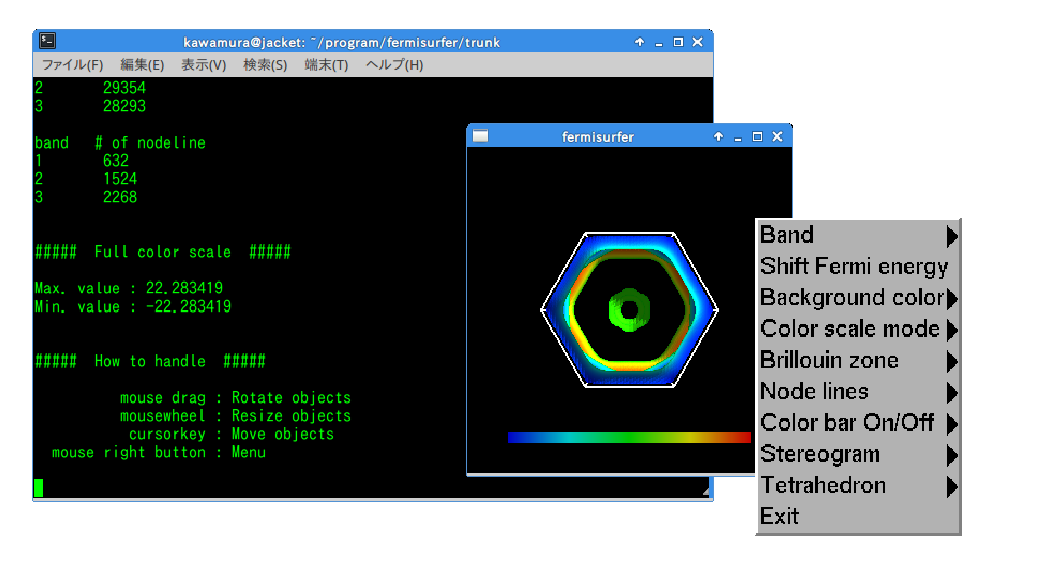
\includegraphics[width=17cm]{figs/start.eps}
  \caption{.}
  \label{fig_start}
\end{figure}

The following operations are available:
\begin{itemize}
\item Rotation of objects with mouse drag
\item Expand and shrink with mouse wheel
\item Window re-sizing
\item Moving objects with cursor keys
\item Opening the menu with mouse right button
\end{itemize}

Here, I will explain all menus.

\subsection{Band}

It makes each band enable/disable (Fig. \ref{fig_band}).

\begin{figure}[!ht]
  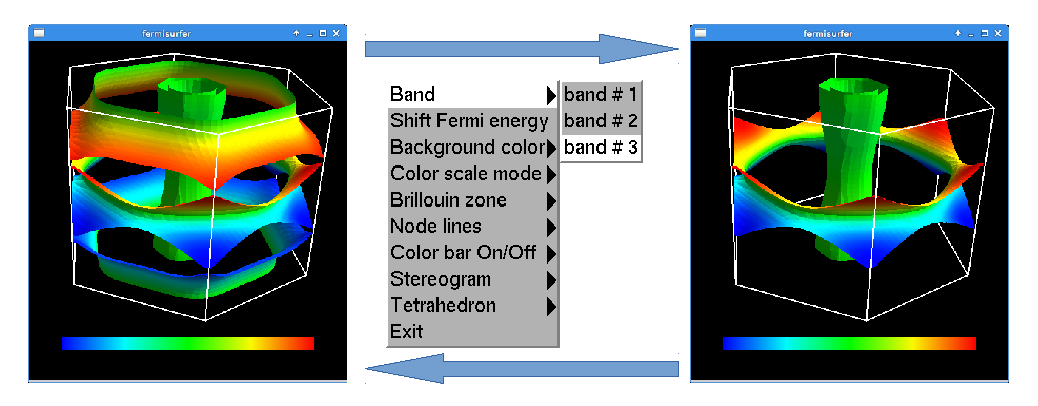
\includegraphics[width=17cm]{figs/band.eps}
  \caption{You make each band enable/disable with \texttt{Band} menu.}
  \label{fig_band}
\end{figure}

\subsection{Shift Fermi energy}

It shifts the Fermi energy (= 0 in default) to arbitrary value.
When you use this menu, 
first, it displays minimum and maximum energy in the input file
and the current Fermi energy;
\begin{verbatim}
Min  Max  E_F 
-0.428153 0.497620 0.000000 
Fermi energy shift : 
\end{verbatim}
Then, you should type the new Fermi energy;
finally, the new Fermi surfaces are depicted (Fig. \ref{fig_shift}).

\begin{figure}[!ht]
  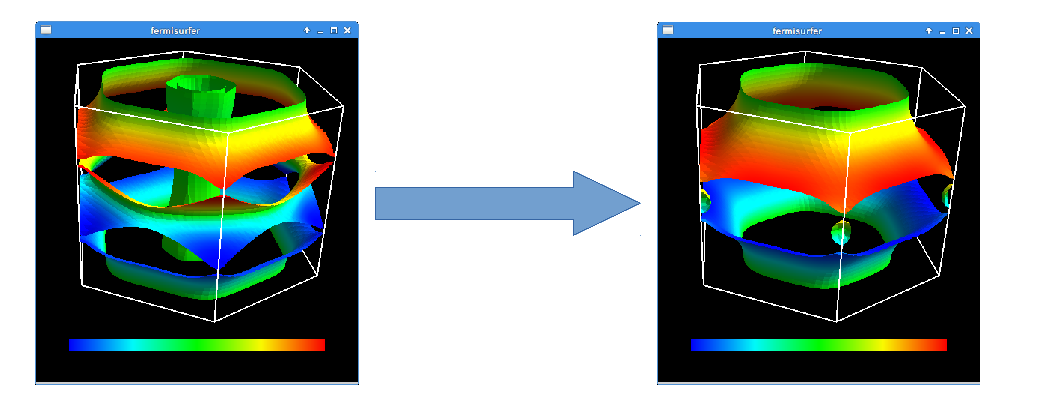
\includegraphics[width=17cm]{figs/shift.eps}
  \caption{The Fermi energy is set from 0 Ry to 0.1 Ry 
    with \texttt{Shift Fermi energy} menu}
  \label{fig_shift}
\end{figure}

\newpage

\subsection{Background color}

The background color is toggled between black and white;
The edge of the Brillouin Zone is also toggled 
between white and black (Fig. \ref{fig_background}). 

\begin{figure}[!ht]
  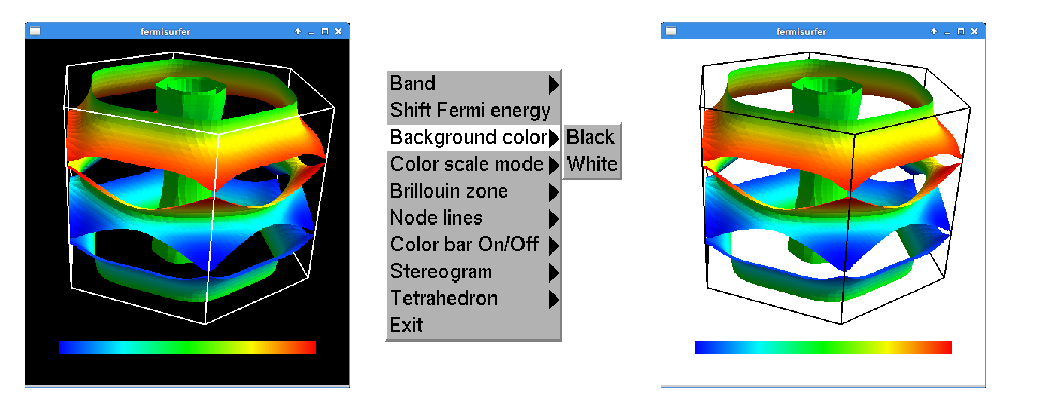
\includegraphics[width=17cm]{figs/background.eps}
  \caption{The background color is toggled with \texttt{Background color} menu.}
  \label{fig_background}
\end{figure}

\subsection{Color scale mode}

It turns color pattern on Fermi surfaces (Fig. \ref{fig_colorscale}). 
\begin{description}
\item[Auto(default)] 
  It makes blue as the minimum on Fermi surfaces and
  red as the maximum on them.
\item[Manual] You can set manually (from standard input) 
  values corresponding to blue and red.
\item[Uni-color] Fermi surfaces of each band are depicted with uni-color
  without relation to the matrix element.
\item[Periodic] It makes periodic color plot enable.
  When the matrix element varies as 
  $0 \rightarrow \pi/3 \rightarrow 2\pi/3 \rightarrow \pi \rightarrow 
  4\pi/3 \rightarrow 5\pi/3 \rightarrow 2\pi$,
  the color varies as 
  red $\rightarrow$ yellow $\rightarrow$ green $\rightarrow$
  cyan $\rightarrow$ blue $\rightarrow$ magenta $\rightarrow$ red. 
\end{description}

\begin{figure}[!ht]
  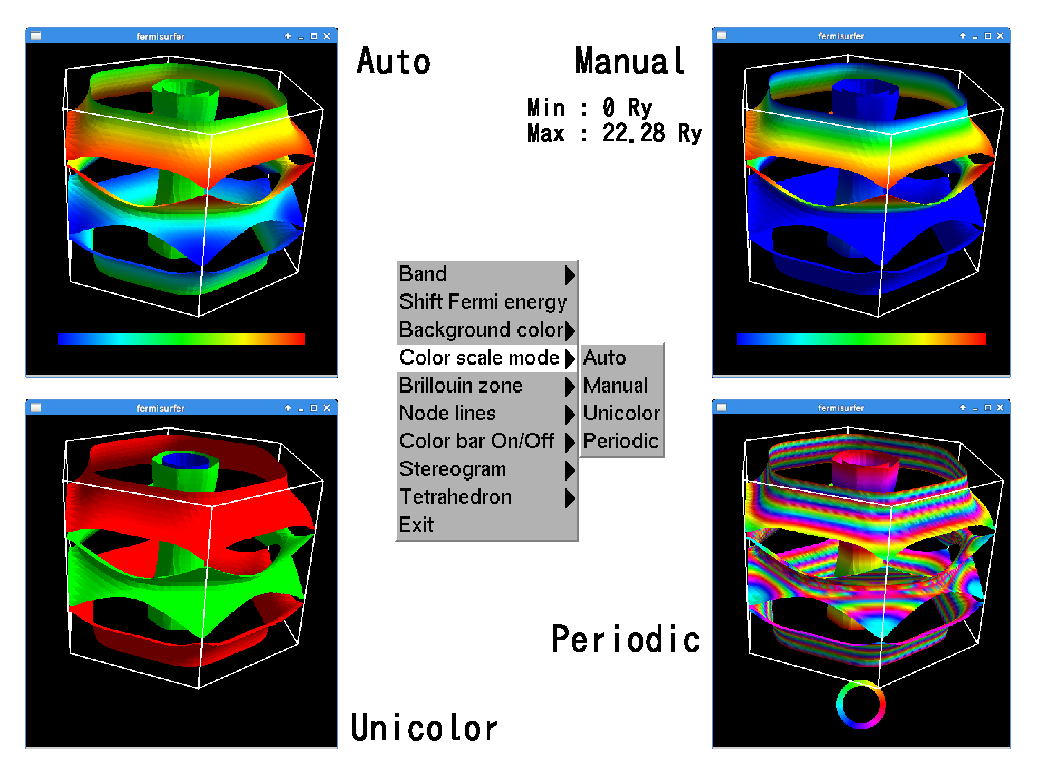
\includegraphics[width=17cm]{figs/colorscale.eps}
  \caption{\texttt{Color scale mode} menu.}
  \label{fig_colorscale}
\end{figure}

\subsection{Brillouin zone}

You choose Brillouin-zone type as follows (Fig. \ref{fig_brillouinzone}): 
\begin{description}
\item[First Brillouin Zone] The region surrounded by Bragg's planes
  the nearest to ${\rm \Gamma}$ point.
\item[Primitive Brillouin Zone] A hexahedron 
  whose corner is the reciprocal lattice point.
\end{description}

\begin{figure}[!ht]
  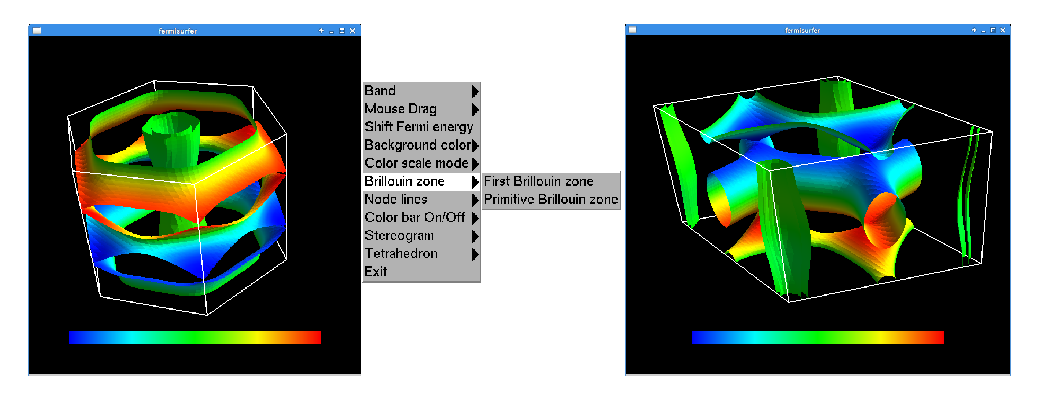
\includegraphics[width=17cm]{figs/brillouinzone.eps}
  \caption{You can change the type of the Brillouin zone 
    with \texttt{Brillouin zone} menu.}
  \label{fig_brillouinzone}
\end{figure}

\newpage

\subsection{Node line}

The line on which the matrix element becomes 0 (we call it node line)
becomes enable/disable (Fig. \ref{fig_nodeline}).

\begin{figure}[!ht]
  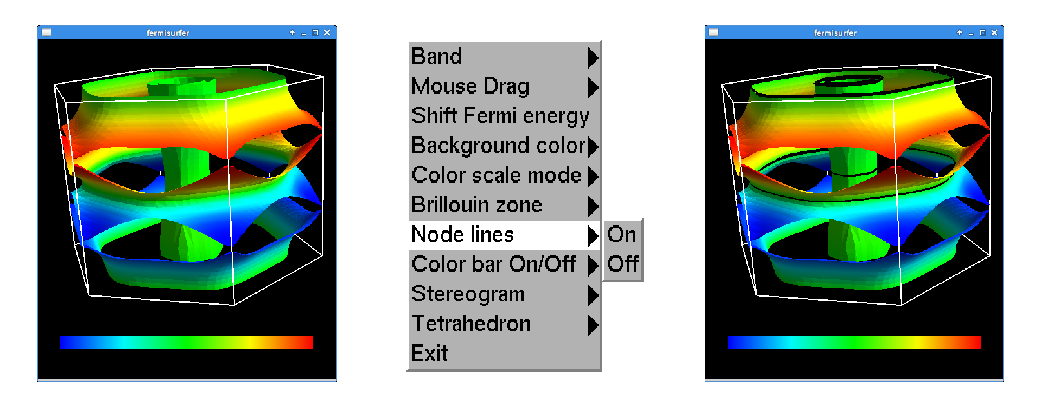
\includegraphics[width=17cm]{figs/nodeline.eps}
  \caption{Toggling the node line with \texttt{Node line} menu.}
  \label{fig_nodeline}
\end{figure}

\subsection{Color bar On/Off}

The color bar becomes enable/disable (Fig. \ref{fig_colorbar}). 

\begin{figure}[!ht]
  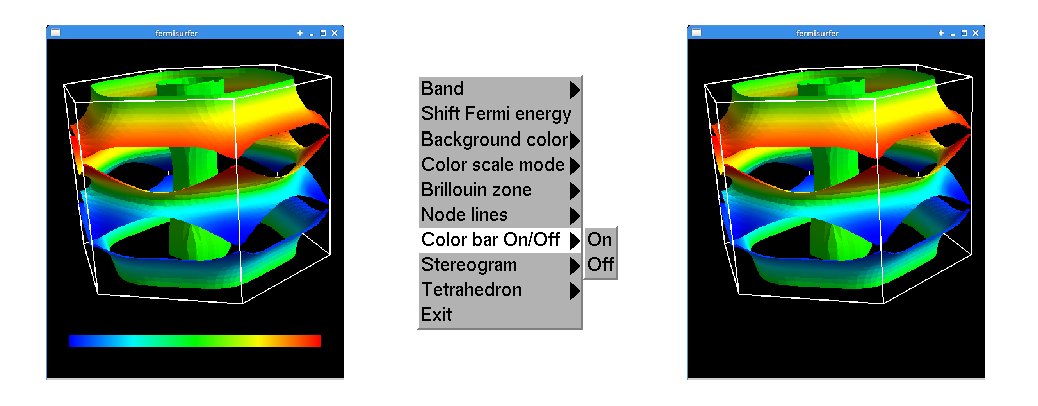
\includegraphics[width=17cm]{figs/colorbar.eps}
  \caption{Toggling the color bar with \texttt{Color bar On/Off} menu.}
  \label{fig_colorbar}
\end{figure}

\subsection{Stereogram}

The stereogram (parallel eyes and  cross eyes) becomes 
enabled/disabled (Fig. \ref{fig_stereogram}).
\begin{description}
\item[None (Default)]   
\item[Parallel] Parallel-eyes stereogram 
\item[Cross] Cross-eyes stereogram 
\end{description}

\begin{figure}[!ht]
  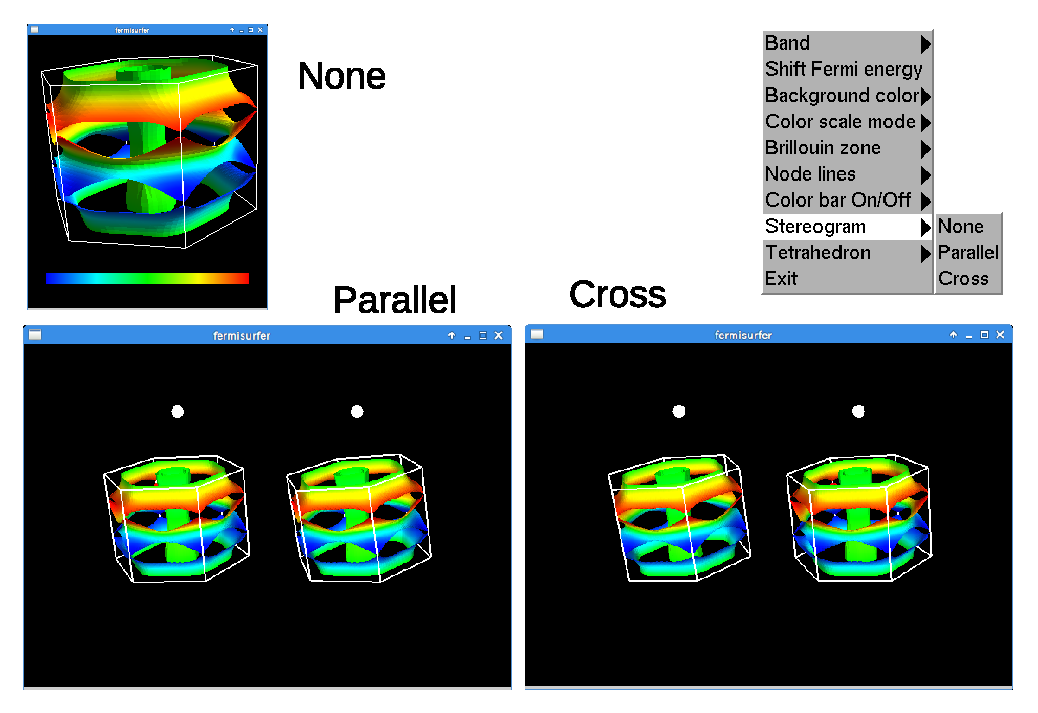
\includegraphics[width=17cm]{figs/stereogram.eps}
  \caption{The stereogram becomes enabled/disabled with \texttt{Stereogram} menu.}
  \label{fig_stereogram}
\end{figure}

\subsection{Tetrahedron}

You change the scheme to divide into tetrahedra (\texttt{tetra \# 1} as default).
It is experimental.

\subsection{Exit}

This finishes \verb|fermisurfer|.

\section{Garally}

Contributions of each Fermi surfaces to the Hall effect
in IrO$_2$
(Fig. \ref{fig_iro2}. Provided by Mr. Wataru Sano in Arita group, RIKEN)

\begin{figure}[!ht]
  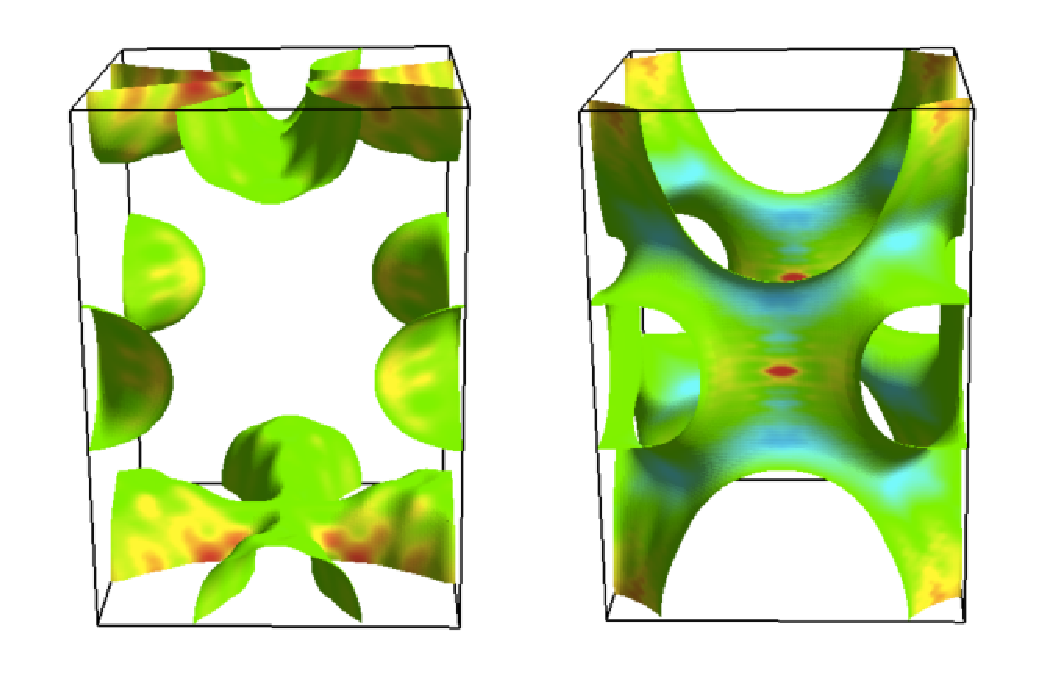
\includegraphics[width=17cm]{figs/iro2.eps}
  \caption{Contributions of each Fermi surfaces to the Hall effect}
  \label{fig_iro2}
\end{figure}

\end{document}
